\chapter{Introduction}
\label{ch:introduction}
As new applications are found the performance required from processors increases. This increase used to be gained primarily by increasing the clock speed of the processor. From 1987 to 2003 processor clock speed increased on average by 40\% per year, shown in Figure \ref{fig:CPUSPEED}, which was achieved by reducing transistor size, leading to decreased propagation delays but has the side effect of increasing power density.

\begin{figure}[h]
	\centering
	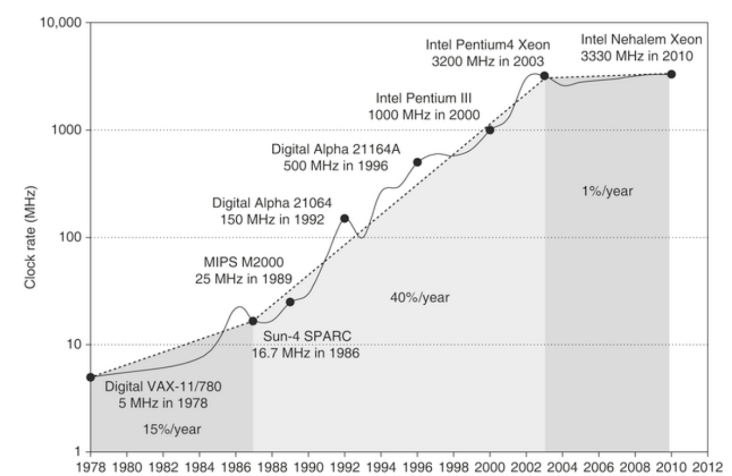
\includegraphics[width=0.8\textwidth]{CPU_clock_speed.png}
	\caption{Graph showing trends in clock speed growth \cite[Figure~1.11] {CPUSPEED}}
	\label{fig:CPUSPEED}
\end{figure}

Issues are found when a limit is reached where the physical materials on the chip can not dissipate the heat faster than it is generated. From 2003 a drastic decrease in yearly clock speed gains showing the impact of this limit can be seen in Figure \ref{fig:PROCTREND}. Instead processor manufacturers started increasing core count to allow the use of parallelism for performance gain. General purpose parallelism is beneficial but has diminishing returns due to the ability of applications to harness multiple cores and the size requirements to add more cores. Another option is to use specificity designed hardware accelerators that can fully exploit the massive parallelism inherent in many different applications. Hardware accelerators also eliminate overhead such as the fetch\mbox{-}decode\mbox{-}execute cycle that is needed by a processor which can increase power efficiency.

\begin{figure}[h]
	\centering
	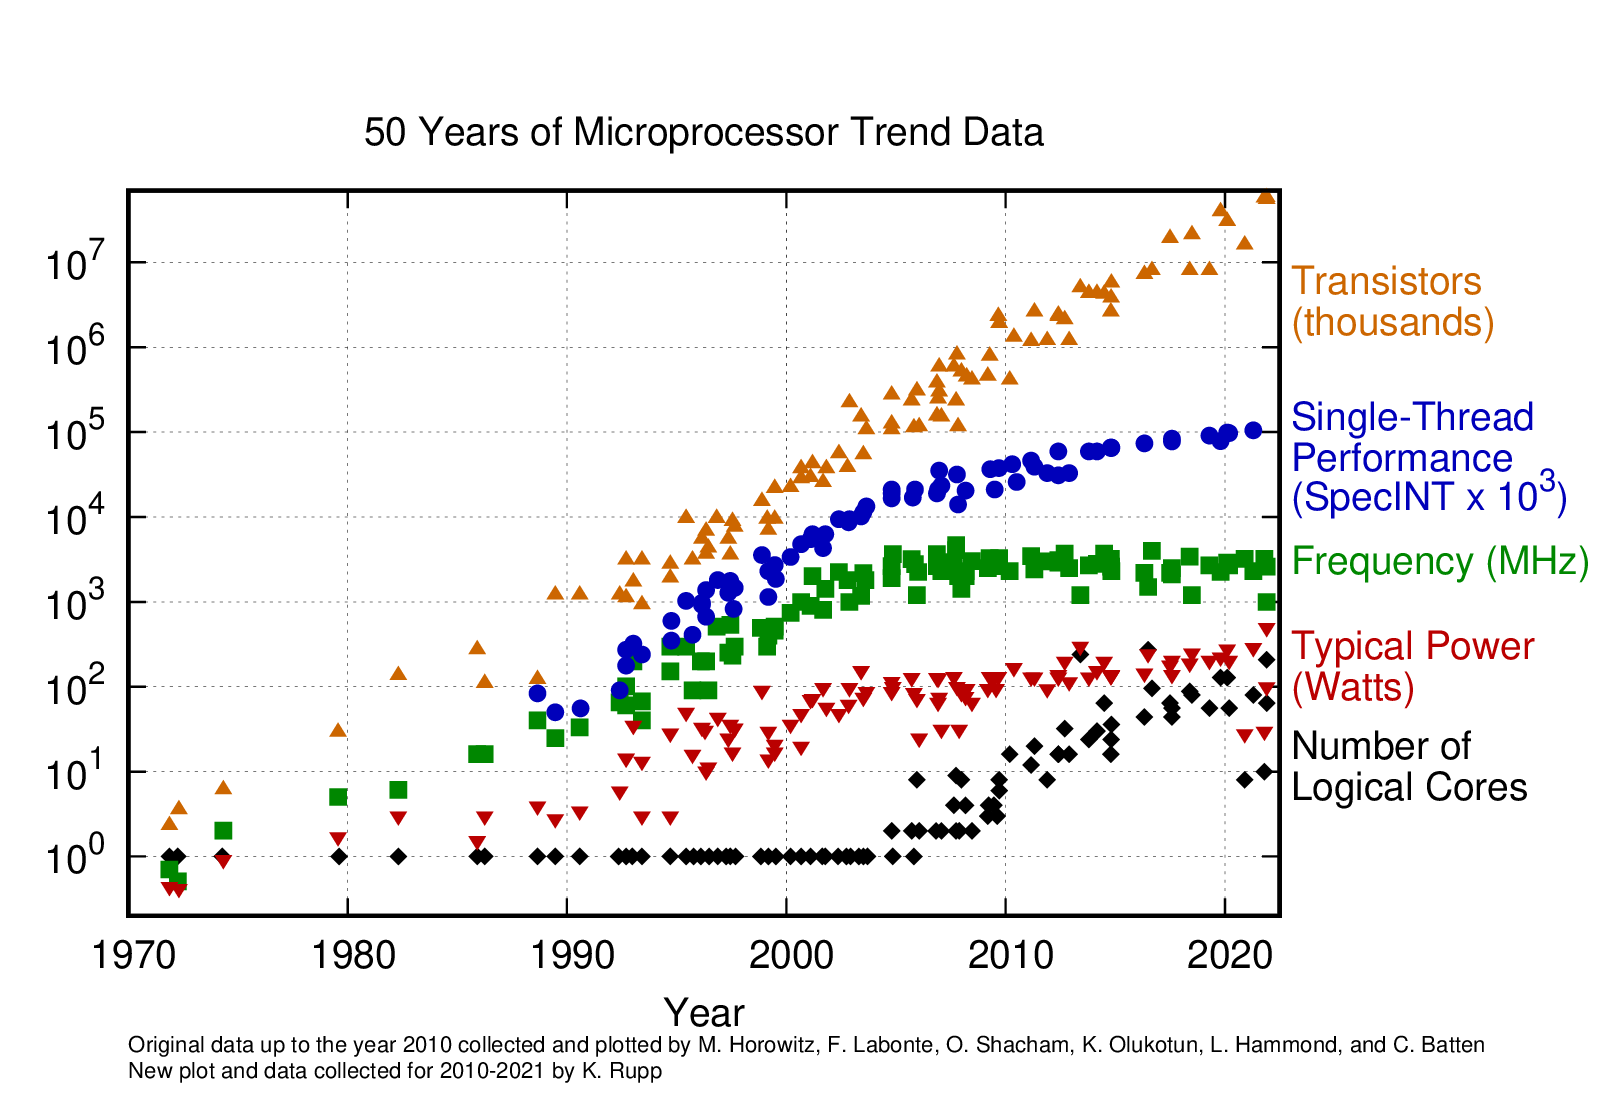
\includegraphics[width=0.8\textwidth]{50-years-processor-trend.png}
	\caption{rends in processors transistor count, clock speed, power usage and core count \cite{PROCTREND}}
	\label{fig:PROCTREND}
\end{figure}

One application for which hardware acceleration could be used is the execution of Cellular Automata (CA) which is a method of modelling complex phenomena based on simple rules. CA execution can utilize massive parallelisation as all calculations are independent, creating the possibility of constant time computation if sufficiently parallelised.

As these hardware accelerators are physical devices, development and iterations of designs can be slow and expensive if the hardware must be physically constructed each time. Field\mbox{-}Programmable Gate Arrays (FPGAs) provide a solution to this problem by providing a form of reconfigurable hardware that can be programmed to implement any design \cite{WHATISFPGA}. This project will use an FPGA chip to develop a CA hardware accelerator for a processor that can be used to evaluate the benefits of dedicated hardware.

RISC\mbox{-}V is an open standard instruction set architecture (ISA) that can be implemented when designing a processor \cite{RISCV}. Due to its open nature this ISA, has seen wide spread adoption in both high\mbox{-}performance products, such as SiFive boards, and in low\mbox{-}power microcontrollers such as Espressif’s ESP32\mbox{-}C3. There is also an FPGA implementation \cite{Asanović:EECS-2016-17} that can be modified and extended to add extra functionality. This provides an excellent foundation for this project to build off of as any developments would be just as applicable in the many real world application that utilize RISC\mbox{-}V.

\section{Objectives}
\label{sec:objectives}

This project will develop a cellular automata hardware accelerator integrated into a RISC\mbox{-}V processor and evaluate it’s performance when compared to other methods of execution. Below is a list of objectives for this project.

\begin{enumerate}
	\item Generate and implement a RISC\mbox{-}V core on the FPGA that can run bare\mbox{-}metal code.
	\item Develop hardware that can be integrated into the processor so data can be written to and read from the accelerator.
	\item Develop hardware than can perform CA computations utilizing the inherent parallelisation of the application.
	\item Implement a bare\mbox{-}metal driver for the hardware accelerator.
	\item Evaluate the performance of the accelerator compared to computation through bare\mbox{-}metal code.
\end{enumerate}